\documentclass{beamer}
\usetheme{Madrid}
\usepackage{minted}
% sudo tlmgr install minted
\usepackage[utf8]{inputenc}
\usepackage[T2A]{fontenc}
\usepackage[russian,english]{babel}

% Footline: show current section (left) and frame numbers (right)
\setbeamertemplate{footline}{%
  \leavevmode%
  \hbox{%
    \begin{beamercolorbox}[wd=.78\paperwidth,ht=2.5ex,dp=1ex,left]{author in head/foot}%
      \hspace*{1em}\usebeamerfont{footline}\insertsectionhead%
    \end{beamercolorbox}%
    \begin{beamercolorbox}[wd=.22\paperwidth,ht=2.5ex,dp=1ex,right]{date in head/foot}%
      \usebeamerfont{footline}\insertframenumber{} / \inserttotalframenumber\hspace*{1em}%
    \end{beamercolorbox}%
  }%
}

\newcommand{\parpause}[1]{\only<+->{#1\par}}

\AtBeginSection[]
{
  \begin{frame}
    \frametitle{Содержание}
    \tableofcontents[currentsection]
  \end{frame}
}

\title{Семинар 2. Часы и время в распределенных системах}
\subtitle{Распределенные вычисления}
\author{Георгий Семенов}
\institute{Институт прикладных компьютерных наук \\ Университет ИТМО}
\date{весна 2026}

\begin{document}

\frame{\titlepage}

\begin{frame}
\frametitle{Организационные моменты}

\begin{itemize}
  \item Материалы семинаров и домашек появились на GitHub
  \item Есть вероятность, что первая домашка будет посвящена часам! (о них – сегодня)
\end{itemize}

\end{frame}

\section{Время в распределенных системах}

\begin{frame}{Время как проблема}
\begin{itemize}
\item В распределённой системе нет глобальных часов: разные узлы, разные ядра процессора, разный <<пульс времени>>
\item Время передачи сообщений в общем случае неизвестно и может быть большим (пример с ping)
\item Еще хуже – физические часы дрейфуют ($\pm \epsilon$)
\end{itemize}

\textbf{Вопрос:} как определить, какое событие произошло раньше?
В идеальном случае хочется:

\begin{itemize}
\item Монотонность – <<время течет всегда вперед>>
\item Согласованность – если $a$ произошло до $b$, то $t(a) < t(b)$
\item Уникальность – разные события имеют различимые метки времени
\end{itemize}

\end{frame}


\begin{frame}{Два типа времени}
\begin{block}{Тотально упорядоченно (total order, linear, wall-clock, linerializble)}
Любые два события сравнимы $<$: до или после (иррефлексивное, транзитивное, антисимметричное).
\end{block}

\begin{block}{Частично упорядоченное (partial order, causal, logical, concurrent)}
Некоторые события несравнимы $<$: до, после или конкурентно (иррефлексивное, транзитивное, антисимметричное).
\end{block}

Физическое время $\Rightarrow$ тотальный порядок \\
Причинность $\Rightarrow$ частичный порядок

\end{frame}

\section{Часы реального времени и алгоритмы синхронизации}

\begin{frame}{Real-Time Clock}

Модель реального времени (физические часы) – это функция $C(t)$, которая отображает реальное время $t$ в метку времени $C$.

\[
C(t) = t + \epsilon(t)
\]

где $\epsilon(t)$ — ошибка.

Два параметра:
\begin{itemize}
\item \textbf{Drift} — отклонение скорости (разность тактовой частоты от эталона)
\item \textbf{Skew} — разница между часами (относительный сдвиг)
\end{itemize}
\end{frame}

\begin{frame}{Как дела обстояли на материнской плате?}

\begin{center}
  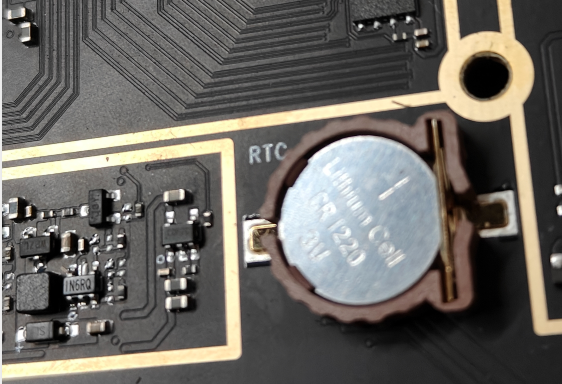
\includegraphics[width=1.0\linewidth,keepaspectratio]{images/rtc_motherboard.png}
\end{center}

\end{frame}


\begin{frame}{Синхронизация часов}
\textbf{Cristian's algorithm (1989)}
\begin{itemize}
\item Осуществляем Round-Trip с запросом времени
\item Вычисляем сдвиг как временной сдвиг между клиентом и сервером: $RTT / 2$
\item В чем недостаток алгоритма? % не монотонное время, наивное предположение о симметричности (и соответственно, времени запроса и ответа) канала
\end{itemize}


\textbf{Berkeley algorithm (1989)}
\begin{itemize}
\item Делегируем быть <<часовщиком>> одному узлу системы (через leader election)
\item Как в прошлом алгоритме, собираем и оцениваем время на узлах (включая себя) через Round-Trip
\item Усредняем и сообщаем всем узлам, какой offset им надо к себе прибавить
\end{itemize}
\end{frame}


\begin{frame}
\frametitle{Алгоритм Кристиана}

Алгоритм Кристиана – алгоритм синхронизации времени между клиентом и временным сервером.

\textbf{Идея:} клиент отправляет запрос серверу времени и корректирует своё локальное время на основе полученного ответа.

\vspace{0.3cm}

\textbf{Процесс:}
\begin{enumerate}
  \item Клиент отправляет запрос серверу времени в момент $T_0$ (по его часам)
  \item Сервер отвечает со своим временем $T_s$
  \item Клиент получает ответ в момент $T_1$ (по его часам)
\end{enumerate}

\vspace{0.3cm}

\textbf{Оценка задержки и коррекция:}

Время в пути туда и обратно: $RTT = T_1 - T_0$

Предполагаемое время в пути в одну сторону: $\delta = \frac{RTT}{2}$

Скорректированное время сервера: $T_s + \delta$

\vspace{0.3cm}

\textbf{Оценка ошибки:} Максимальная ошибка синхронизации: $\pm\delta = \pm\frac{RTT}{2}$

\end{frame}


\begin{frame}{NTP}
Network Time Protocol – семейство алгоритмов с поддержкой масштабируемости:

\begin{itemize}
\item Round-Trip с оценкой корректировки (алгоритм Marzullo)
\item Иерархия страт (stratum 0 – эталонные часы)
\item Точность – миллисекунды (Интернет), микросекунды (LAN)
\end{itemize}

\begin{center}
  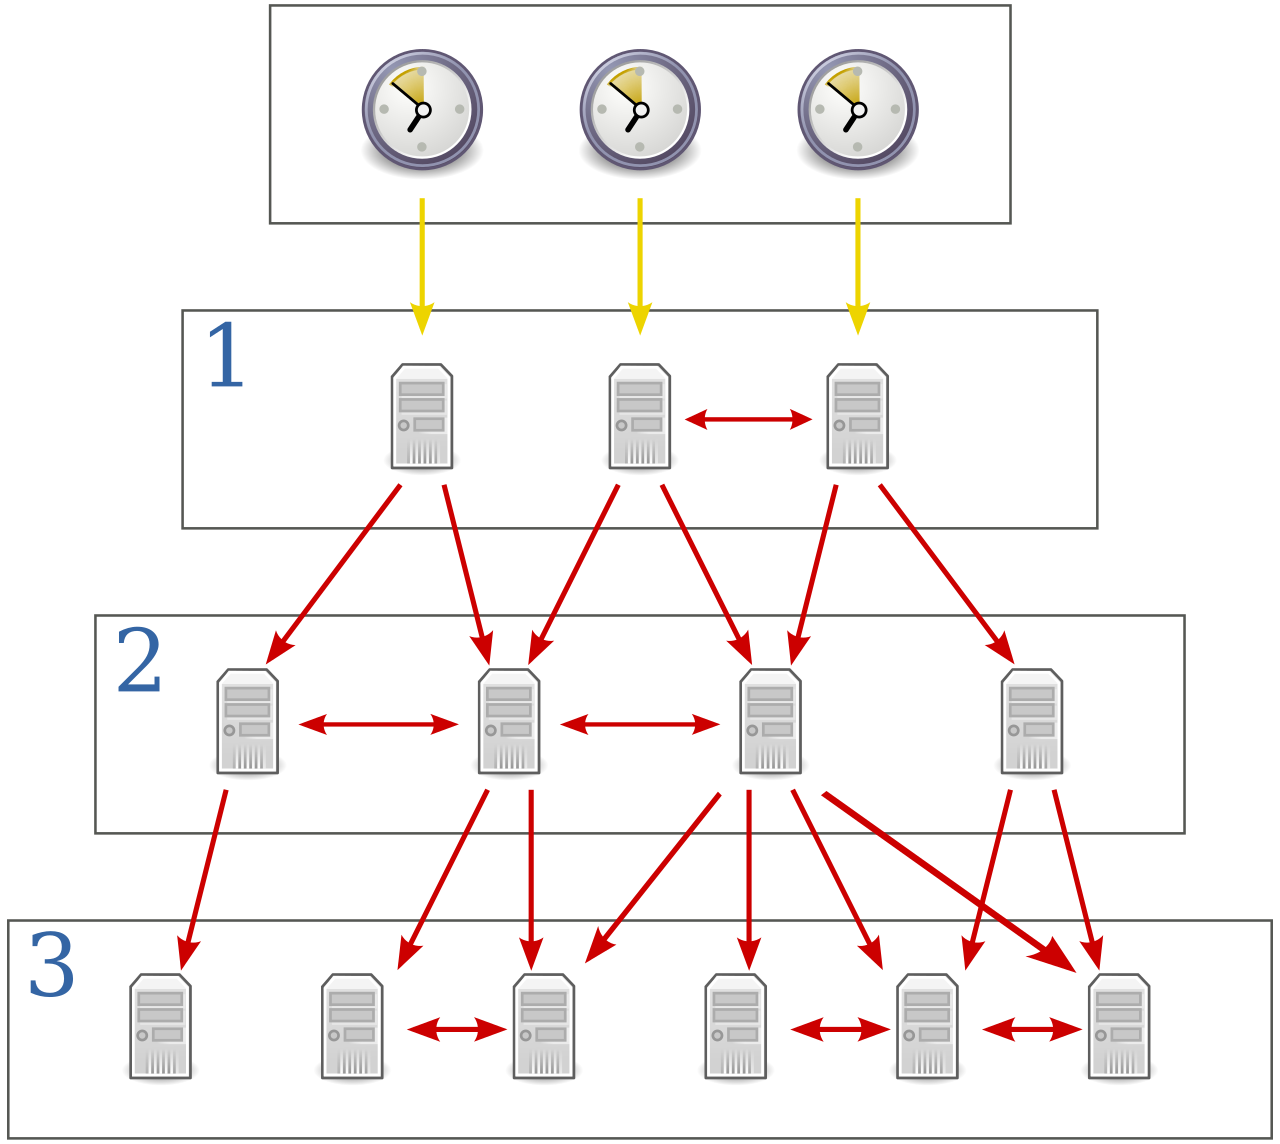
\includegraphics[width=0.5\linewidth,keepaspectratio]{images/NTP.png}
\end{center}

\end{frame}

\begin{frame}{TrueTime (Google Spanner)}
Идея:

\[
TT.now() = [earliest, latest]
\]

Время задаётся интервалом неопределённости.

Позволяет:
\begin{itemize}
\item обеспечить внешнюю консистентность
\item реализовать commit-wait
\end{itemize}
\end{frame}

\section{Монотонные часы}

\begin{frame}{Monotonic Clock}
Требование:

\[
t_2 > t_1 \Rightarrow C(t_2) \ge C(t_1)
\]


Используется для:
\begin{itemize}
\item измерения интервалов
\item таймаутов
\item backoff
\end{itemize}
\end{frame}


\begin{frame}{Модель времени в C++}
\texttt{std::chrono::system\_clock}
\begin{itemize}
\item отражает wall-clock
\item может изменяться назад
\end{itemize}


\texttt{std::chrono::steady\_clock}
\begin{itemize}
\item монотонный
\item не связан с календарным временем
\item не гарантирована синхронизация между машинами
\end{itemize}
\end{frame}

\section{Частично упорядоченное время и логические часы}

\begin{frame}{Lamport (1978)}
Статья:
\textit{Time, Clocks, and the Ordering of Events in a Distributed System}

Главная идея:
\begin{center}
\textbf{Время = причинность}
\end{center}

\begin{center}
  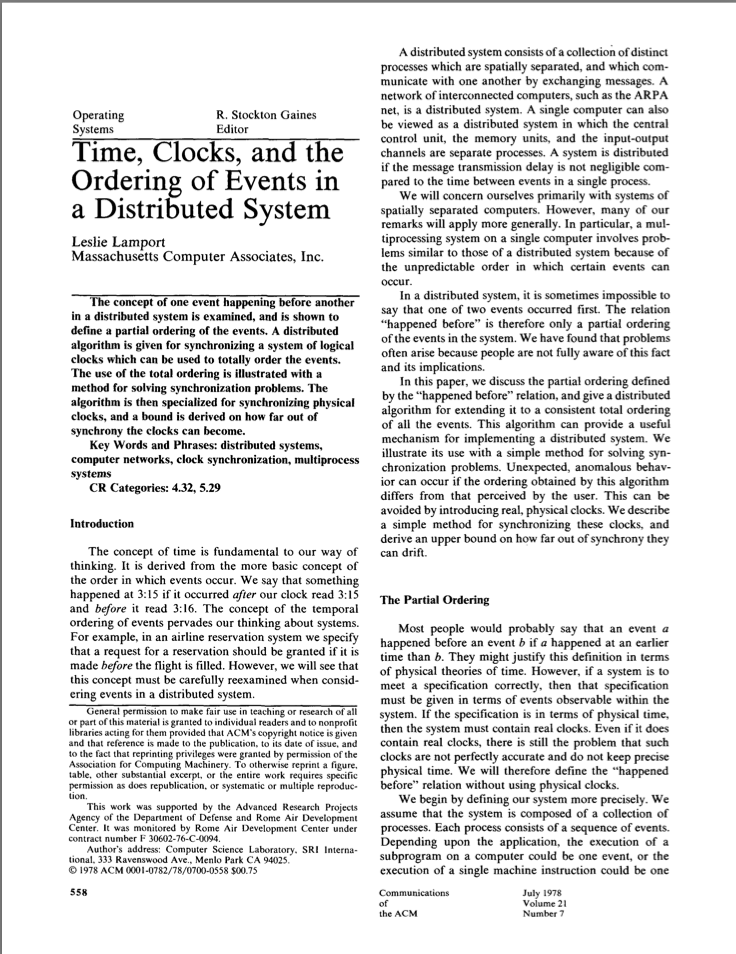
\includegraphics[width=0.8\linewidth,keepaspectratio]{images/lamport_time_paper.png}
\end{center}

\end{frame}

\begin{frame}{Отношение happens-before}
Определение:

$a \rightarrow b$, если:

\begin{enumerate}
\item События в одном процессе и $a$ раньше $b$
\item $a$ — отправка, $b$ — получение сообщения
\item Транзитивность
\end{enumerate}

\begin{block}{Тотально упорядоченное время}
\[
    \forall a, b: a \rightarrow b \Leftrightarrow t(a) < t(b)
\]
\end{block}

\begin{block}{Частично упорядоченное время}
\[
    \forall a, b: a \rightarrow b \Rightarrow t(a) < t(b)
\]
\end{block}

\end{frame}


\begin{frame}{Часы Лампорта}

  Интуиция:
  \begin{itemize}
    \item "ничто на Земле не проходит бесследно"
    \item если произошло $B$, и $A$ happens-before $B$, то это должно привести к <<утечке>> времени, т.е. $L(A) < L(B)$
  \end{itemize}

  % Иными словами, существует два фундаментальных типа событий, отражающих отношение happens-before:
  % \begin{itemize}
  %   \item Создание события внутри одного процесса (на нем тотальное время)
  %   \item Отправка и получение сообщения между процессами (передача события)
  % \end{itemize}

Алгоритм для каждого процесса $P$ с локальной переменной $C$:

\begin{enumerate}

\item Когда хочу создать событие:
  \begin{itemize}
    \item Добавлю в событие метку, соответствующую моим текущим часам: $L := C$
    \item Атомарно инкрементирую свои часы на единицу: $C := C + 1$
  \end{itemize}

\item Когда получаю чужое событие:
  \begin{itemize}
    \item Обновляю свои часы: $C := \max(C, C_m) + 1$
  \end{itemize}

\end{enumerate}
\end{frame}


\begin{frame}{Иллюстрация часов Лампорта}
% https://dis.dankook.ac.kr/lectures/dms16/2016/05/21/lamport-vs-vector-clock/

\begin{center}
  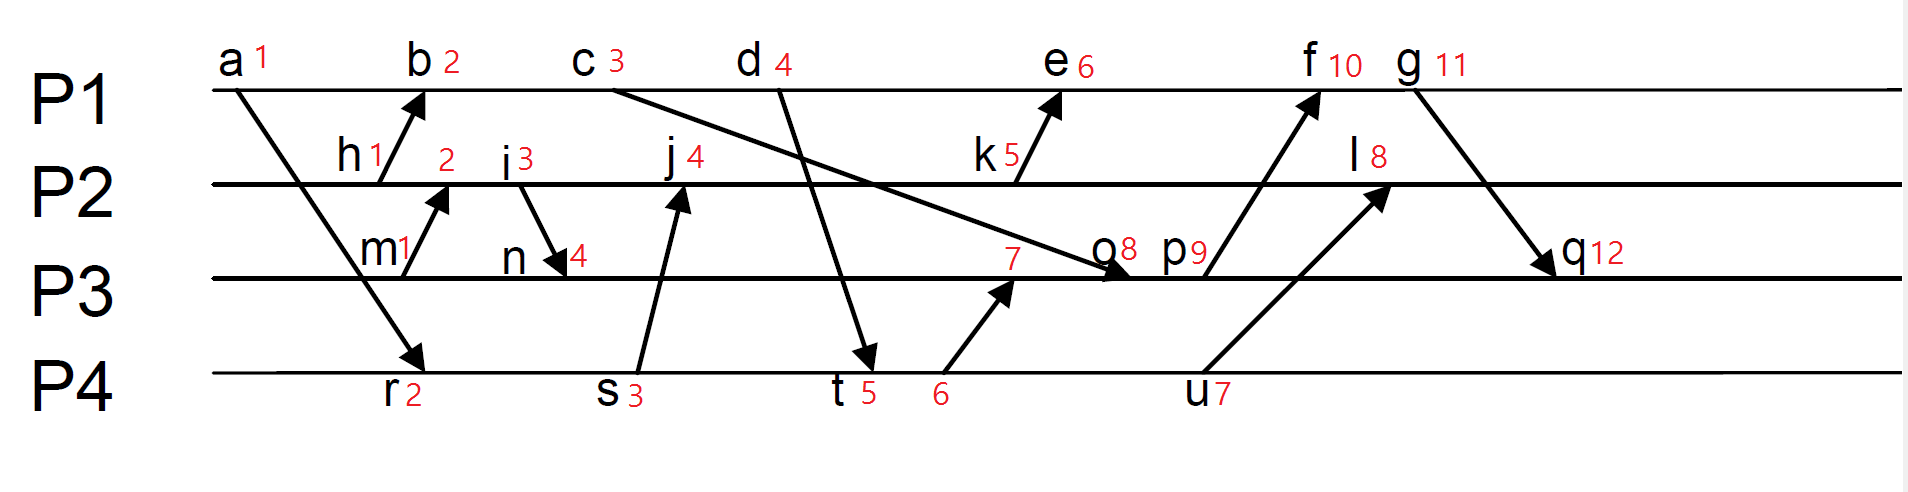
\includegraphics[width=1.0\linewidth,keepaspectratio]{images/Lamport-Clock-Timestamp.png}
\end{center}

(!) Часы Лампорта не позволяет причинную связь между событиями!

Они лишь позволяют понять следующее:

\[ L(A) \geq L(B) \Rightarrow A \not\rightarrow B \]


\end{frame}


\begin{frame}{Векторные часы}
Каждый процесс хранит вектор размера $N$ с текущей известной меткой времени, происходящего
на каждом из процессов:

\begin{enumerate}

\item Когда хочу создать событие:
  \begin{itemize}
    \item Добавлю в событие метку, соответствующую моим текущим часам: $L := C[i]$
    \item Атомарно инкрементирую свои часы на единицу: $C[i] := C[i] + 1$
  \end{itemize}

\item Когда получаю чужое событие:
  \begin{itemize}
    \item Обновляю свои часы: $\forall j: C[j] := \max(C[j], C_m[j])$
    \item Атомарно инкрементирую свои часы на единицу: $C[i] := C[i] + 1$
  \end{itemize}
\end{enumerate}

\end{frame}


\begin{frame}{Иллюстрация векторных часов}
% https://dis.dankook.ac.kr/lectures/dms16/2016/05/21/lamport-vs-vector-clock/

\begin{center}
  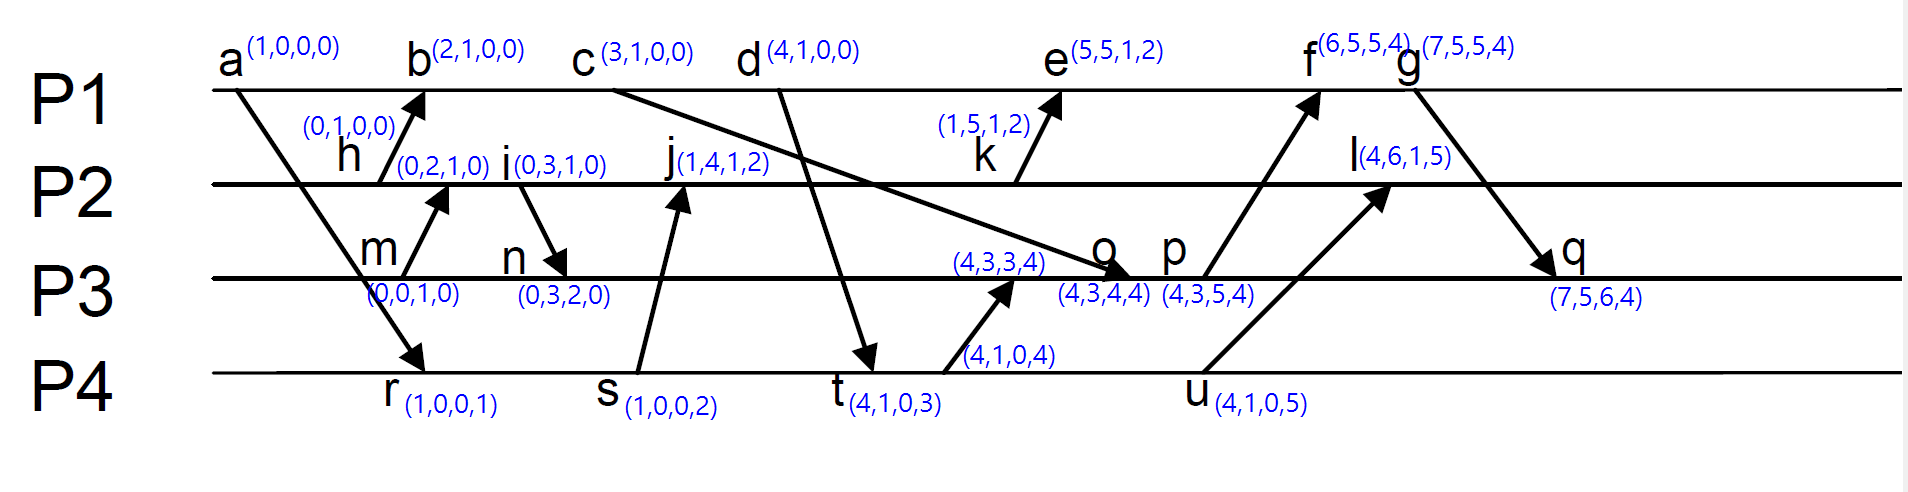
\includegraphics[width=1.0\linewidth,keepaspectratio]{images/Vector-Clock-Timestamps.png}
\end{center}

Как определяется отношение happens-before между векторными часами $A$ и $B$?

\[
A \rightarrow B \Leftrightarrow \forall i: A[i] \leq B[i] \text{ и } \exists i: A[i] < B[i]
\]

\[
A \parallel B \Leftrightarrow \exists i: A[i] > B[i] \text{ и } \exists i: A[i] < B[i]
\]

\end{frame}

\begin{frame}{Минимальность}

Векторные часы — минимальное точное представление
частичного порядка в общем случае (Charron-Bost, "Concerning the size of clocks", 1990)

\begin{itemize}
\item Causal consistency: доставка сообщений в порядке причинности
\item CRDT: операции, которые могут быть применены в любом порядке, но результат будет одинаковым
\item Отслеживание конфликтов: два параллельных события могут привести к конфликту, который нужно разрешить
\item Distributed debugging/tracing/thread sanitizer
\end{itemize}

\end{frame}


\begin{frame}{Итоги}
\begin{itemize}
\item Время – то, что позволяет нам рассуждать о событиях внутри распределенной системы
\item В зависимости от порядка событий мы можем говорить о разных состояниях системы
\item Физическое время – привычно нам, но оно не обладает монотонностью
\item Логическое время – относительная конструкция, но с ней можно рассуждать о причинности
\end{itemize}
\end{frame}


\begin{frame}{Блогопосты, чтобы разобраться лучше}
\begin{enumerate}
\item \href{https://sookocheff.com/post/time/lamport-clock/}{Kevin Sookocheff. Lamport Clocks}
\item \href{https://martinfowler.com/articles/patterns-of-distributed-systems/lamport-clock.html}{Martin Fowler. Lamport Clocks}
\item \href{https://www.geeksforgeeks.org/dsa/lamports-logical-clock/}{GeeksforGeeks. Lamport's Logical Clock}
\item \href{https://mwhittaker.github.io/blog/lamports_logical_clocks/}{Michael Whittaker. Lamport's Logical Clocks}
\item \href{https://sookocheff.com/post/time/vector-clocks/}{Kevin Sookocheff. Vector Clocks}
\item \href{https://medium.com/@balrajasubbiah/lamport-clocks-and-vector-clocks-b713db1890d7}{Balraja Subbiah. Lamport Clocks and Vector Clocks}
\end{enumerate}
\end{frame}


\end{document}